\section{The Ellipsoid Method}
\label{sect:ellipsoid-method}
\begin{enumerate}
\item Apart from the (dual) simplex method studied previously, there are also
other algorithms for solving LP problems. A major motivation for developing
these alternative algorithms is that while the simplex method is ``often''
efficient (and hence is indeed widely used for solving LP problems), it could
take ``exponential time'' for some exceptional LP problems. On the other
hand, the \emph{ellipsoid method} (to be discussed in
\Cref{sect:ellipsoid-method}) provides a theoretical guarantee that
LP problems can be solved in ``polynomial time'' (which is ``faster'' than
``exponential time''). While the ellipsoid method is \emph{not} an algorithm
for solving LP problems by itself, such theoretical guarantee does lead to a
new class of algorithms, known as \emph{interior point methods}, which can
solve LP problems efficiently; see \Cref{sect:int-pt-methods}.

\item The phrases ``exponential time'' and ``polynomial time'' mentioned above are
used for describing the efficiency of algorithm. To understand them better, we
will briefly study some related concepts in \Cref{subsect:comp-complexity}; you
may consider taking a computer science course about algorithms (e.g., COMP2119)
for a more detailed discussion on them.
\end{enumerate}
\subsection{Computational Complexity}
\label{subsect:comp-complexity}
\begin{enumerate}
\item \textbf{Basic terminologies.} Here, we shall focus on analyzing the
computational complexity of algorithms for solving optimization problems, which
describes how ``fast'' such algorithms are. We start by defining some related
terms:
\begin{itemize}
\item An \defn{instance} is a pair \((S,f)\) where
\(S\subseteq \R^n\) is the feasible region and \(f:S\to\R\) is the objective function.
\item A \defn{problem} is a collection of instances.
\item An \defn{algorithm} conducts a finite sequence of operations until a
stopping criterion \faIcon[regular]{pause-circle} is reached.
\item The \defn{size} of an instance is the number of parameters used to
describe the instance, according to a prespecified format.
\item The \defn{running time} of an algorithm is the number of arithmetic
operations needed until a stopping criterion \faIcon[regular]{pause-circle} is
reached, which generally depends on the instance.
\item \(T(n)\) denotes the worst-case (longest) running
time of an algorithm over all instances of size \(n\).
\item An algorithm runs in \defn{polynomial time} if there exists \(k\in\N\)
such that \(T(n)=O(n^k)\), where we write \defn{\(f(n)=O(g(n))\)} if there
exist \(n_0\in\N\) and \(c>0\) such that \(f(n)\le cg(n)\) for all \(n\ge
n_0\).

\begin{note}
For our purpose here, we can treat an algorithm that takes exponential time
as one with worst-case runtime growing exponentially in \(n\).
\end{note}
\end{itemize}
Since exponential growth is much quicker than polynomial growth, algorithms
that run in polynomial time are regarded as ``fast'' (compared with
algorithms that take exponential time at least).

Often, enumeration algorithms, i.e., algorithms that examine \emph{every
possible} candidate of optimal solutions, take exponential time.  In the
context of LP, an enumeration algorithm is to compute the objective function
value for every vertex of the feasible region and then compare them. So, while
such enumeration algorithms are quite easy to understand, they are rather
inefficient most of the times.
\item \label{it:iter-algo-poly-time} \textbf{Iterative algorithms.} Many
algorithms are \emph{iterative}, whose operations are grouped into iterations.
For example, the simplex method is an iterative algorithm. For this kind of
algorithms, we have the following criterion for running in polynomial time.

Suppose that each iteration of an algorithm can be completed with
\emph{polynomially many operations} (with respect to the size of instance).
Then, the algorithm runs in polynomial time iff the \emph{number of iterations}
(not operations) needed to solve an arbitrary instance of size \(n\) is
\(O(n^k)\).
\item \textbf{Simplex method takes exponential time.} As mentioned earlier, the
simplex method is an iterative algorithm that takes exponential time. This fact
is established by the following result, which gives us an example where the
simplex method would take exponential time.

\begin{proposition}
\label{prp:simplex-expo-time}
Consider the LP problem
\begin{align*}
\text{min}\quad&-x_n \\
\text{s.t.}\quad&\varepsilon\le x_1\le 1-\varepsilon \\
&\varepsilon x_{i_1}\le x_i\le 1-\varepsilon x_{i-1}\text{ for all \(i=2,\dotsc,n\).}
\end{align*}
\begin{enumerate}
\item The feasible region has \(2^n\) vertices.
\item The vertices can be ordered such that each one is adjacent to and has
lower objective function value than the previous one.
\item There exists a pivoting rule where the simplex method requires
\rc{\(2^n\) iterations} before it terminates.
\end{enumerate}
\end{proposition}
\begin{intuition}
The feasible region is obtained by having \emph{perturbations} on the unit cube
which is defined by the constraints \(0\le x_1,\dotsc,x_n\le 1\). Here, we want
to construct an example where the objective function value decreases
\emph{strictly} when moving a vertex to another (so that it would not be
possible to ``skip'' many vertices and hence ``quite many'' iterations would be
needed), and such perturbations can allow that.
\end{intuition}

\Cref{prp:simplex-expo-time} indicates that the simplex method would take
exponential time, since for \emph{some} pivoting rule, \rc{\(2^n\) iterations}
are needed, which grow exponentially in \(n\). However, it still leaves the
possibility for the existence of some pivoting rule under which the simplex
method can run in polynomial time; whether such pivoting rule exists is still
an (important!) open question.

\begin{note}
While the \emph{worst-case} running time of the simplex method would be
exponential time, in practice the simplex method is still quite efficient
usually, and is a handy tool for solving LP problems.
\end{note}
\end{enumerate}
\subsection{Development of The Ellipsoid Method}
\begin{enumerate}
\item In view of the theoretical inefficiency of the simplex method
(possibility of taking exponential time), next we will study the
\emph{ellipsoid method}, which can solve linear \emph{feasibility} problems
(i.e., deciding whether LP problems are feasible) with integer data in
polynomial time. It serves as the building block for algorithms that
\emph{solve LP problems} in polynomial time (see \Cref{sect:int-pt-methods}).

\item\label{it:ellip-method-geo} \textbf{Geometry of the ellipsoid method.} We start by introducing
geometric concepts related to the ellipsoid method:
\begin{itemize}
\item \(E\subseteq \R^n\) is an \defn{ellipsoid} (centered at \(\vect{z}\)) if it can be expressed as
\(E=E(\vect{z},D):=\{\vect{x}\in\R^n:(\vect{x}-\vect{z})^{T}D^{-1}(\vect{x}-\vect{z})\le 1\}\)
where \(\vect{z}\in\R^n\) and \(D\in\R^{n\times n}\) is positive definite.
\begin{center}
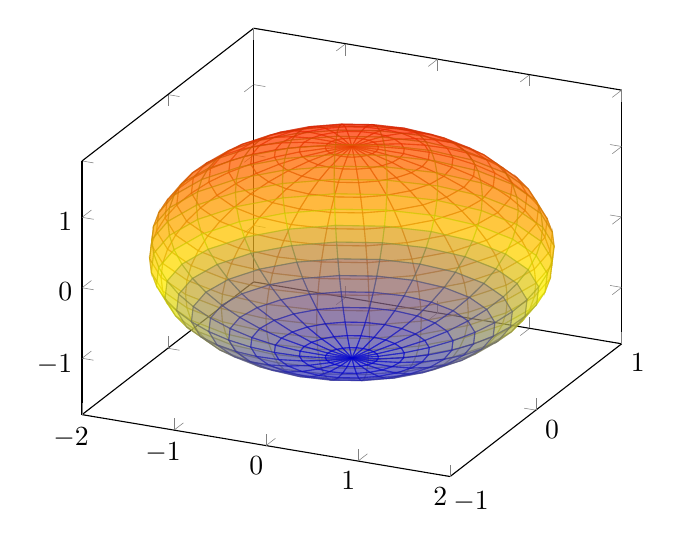
\begin{tikzpicture}
    \begin{axis}[
        domain=0:360,
        domain y=0:180,
    ]
    \addplot3[surf, opacity=0.5]
    (
        {2*cos(x)*sin(y)},
        {1*sin(x)*sin(y)},
        {1.5*cos(y)}
    );
    \end{axis}
\end{tikzpicture}
\end{center}
\begin{remark}
\item \emph{(positive definiteness)} A matrix \(D\in\R^{n\times n}\) is
\defn{positive definite} if it is symmetric and we have
\(\vect{x}^{T}D\vect{x}>0\) for all \(\vect{x}\ne\vect{0}\).
\item \emph{(special case --- ball)} By taking \(D=rI\) with \(r>0\) (check
that it is indeed positive definite!), the ellipsoid \(E(\vect{z},r^{2}I)\)
would become a \emph{ball} centered at \(\vect{z}\) with radius \(r\). From
this, we can see that the notion of \emph{ellipsoid} is a generalization to
\emph{ball}. Indeed, ellipsoid can also be seen as a high-dimensional
generalization to \emph{ellipse} in \(\R^2\).
\end{remark}
\item Let \(D\in\R^{n\times n}\) be an invertible matrix and
\(\vect{b}\in\R^n\). Then the function \(S:\R^n\to\R^n\) defined by
\(S(\vect{x}):=D\vect{x}+\vect{b}\) for all \(\vect{x}\in\R^n\) is called an
\defn{affine transformation}.
\begin{note}
If \(\vect{b}=\vect{0}\), then it becomes a \emph{linear transformation} (the
one from MATH2101). Here, the role of \(\vect{b}\) is \emph{translation} while
the role of \(D\) is \emph{scaling and rotation}.
\end{note}
\item Let \(L\subseteq \R^n\). Then the \defn{volume} of \(L\) is the multiple
integral \(\vol{L}:=\int_{\vect{x}\in L}^{}\odif{\vect{x}}\) (this is the same
as the one from MATH2211).
\end{itemize}
\item \label{it:ellip-method-geo-prop} \textbf{Properties about the
geometrical concepts.} After learning the definitions of the geometrical
concepts in \labelcref{it:ellip-method-geo}, we will study some of
their properties here.
\begin{enumerate}
\item \emph{(characterization of positive definite matrix)} A matrix
\(D\in\R^{n\times n}\) is positive definite iff all of its eigenvalues are
real and positive.
\item \emph{(properties of positive definite matrices)} If \(D\in\R^{n\times
n}\) is positive definite, then:
\begin{enumerate}
\item \emph{(Spectral theorem)} It has a diagonalization \(D=P^{-1}\Lambda P\)
where \(P\) is invertible and \(\Lambda\) is a diagonal matrix with positive
diagonal entries.
\item \(\det{D}=\det{\Lambda}>0\).
\item \(D\) is invertible, and \(D^{-1}\) is positive definite.
\item \(D^{1/2}:=P^{-1}\sqrt{\Lambda}P\) satisfies \(D^{1/2}D^{1/2}=D\), and is
invertible, where \(\sqrt{\Lambda}\) is the diagonal matrix whose each diagonal
entry is the square root of the corresponding one from \(\Lambda\).
\end{enumerate}
\item Let \(B:=\{\vect{x}\in\R^n:\vect{x}^{T}\vect{x}\le 1\}\) be the unit
ball centered at \(\vect{0}\). Then, the ellipsoid \(E(\vect{z},D)\) can be
expressed as \(S(B)\) with the affine transformation
\(S(\vect{x})=D^{1/2}\vect{x}+\vect{z}\).
\item \emph{(volume formula after affine transformation)} Let \(L\subseteq
\R^n\) and \(S(\vect{x})=D\vect{x}+\vect{b}\) be an affine transformation. Then
\(\vol{S(L)}=|\det D|\vol{L}\).

\begin{note}
In particular, this suggests that the volume of the ellipsoid \(E(\vect{z},D)\)
is given by \(\vol{E(\vect{z},D)}=\det D^{1/2}\vol{B}=\sqrt{\det D}\vol{B}\),
where \(\vol{B}\) is the volume of the unit ball.
\end{note}
\end{enumerate}
\begin{pf}
\begin{enumerate}
\item Omitted.
\item Omitted.
\item Note that
\begin{align*}
S(B)&=\{\vect{y}\in\R^n:\vect{y}=D^{1/2}\vect{x}+\vect{z},\vect{x}\in B\}
=\{\vect{y}\in\R^n:(D^{1/2})^{-1}(\vect{y}-\vect{z})\in B\} \\
&=\{\vect{y}\in\R^n:(\vect{y}-\vect{z})^{T}(D^{1/2})^{-1}
(D^{1/2})^{-1}(\vect{y}-\vect{z})\le 1\} \\
&=\{\vect{y}\in\R^n:(\vect{y}-\vect{z})^{T}D^{-1}(\vect{y}-\vect{z})\le 1\}
=E(\vect{z},D).
\end{align*}
\item Using the change-of-variable formula for multiple integral, we have
\[
\vol{S(L)}=\int_{S(L)}^{}\odif{\vect{y}}
=\int_{L}^{}|\det J_{S}(\vect{x})|\odif{\vect{x}}
=\int_{L}^{}|\det D|\odif{\vect{x}}
=|\det D|\vol{L}
\]
where \(J_{S}(\vect{x})\) is the Jacobian matrix of \(S\), which is given by
\(\begin{bmatrix}\pdv{S_1}{x_1}&\cdots&\pdv{S_1}{x_n} \\
\vdots&\ddots&\vdots \\
\pdv{S_n}{x_1}&\cdots&\pdv{S_n}{x_n} \\
\end{bmatrix}=D\).
\end{enumerate}
\end{pf}
\item \textbf{Solving linear feasibility problem by the ellipsoid method.}
With the preparations above, we are now ready to study how to use the ellipsoid
method for solving linear feasibility problem, i.e., given a polyhedron
\(P=\{\vect{x}\in\R^n:A\vect{x}\ge\vect{b}\}\) with \(A\in\R^{m\times n}\) and
\(\vect{b}\in\R^m\), determining whether \(P\) is empty. We start by
introducing the intuitive idea of the ellipsoid method (which is perhaps more
important than the actual implementation details!).

\emph{Intuition:} 
The \underline{ellipsoid} method generates a sequence of
\underline{ellipsoids} \(\{E_t\}\) where the center of \(E_t\) is
\(\vect{x}_t\), such that \(P\subseteq E_t\) for all \(t\). Such sequence of
ellipsoids is obtained in the following iterative process:

For each \(t\):
\begin{enumerate}
\item If \(\vect{x}_t\in P\), then we can immediately deduce that \(P\) is
nonempty and we are done \faIcon[regular]{thumbs-up}.
\item If \(\vect{x}_t\notin P\), then there must exist a constraint that is
violated, so we can write \(\vect{a}^{T}\vect{x}_t<b\) where \(\vect{a}^{T}\)
is a row of \(A\) and \(b\) is the corresponding entry in \(\vect{b}\).
For every \(\vect{x}\in P\), we then have \(\vect{a}^{T}\vect{x}\ge
b>\vect{a}^{T}\vect{x}_t\). Thus, \(P\) is a subset of the halfspace
\(\{\vect{x}\in\R^n:\vect{a}^{T}\vect{x}\ge\vect{a}^{T}\vect{x}_t\}\) which
passes through \(\vect{x}_t\) (``\(=\)'' case), in addition to the
ellipsoid \(E_t\).

\emph{Geometrically}, this means \(P\) is contained in the intersection of the
ellipsoid \(E_t\) and a halfspace that passes through the center of \(E_t\), 
which is said to be a \defn{half-ellipsoid}.
\begin{center}
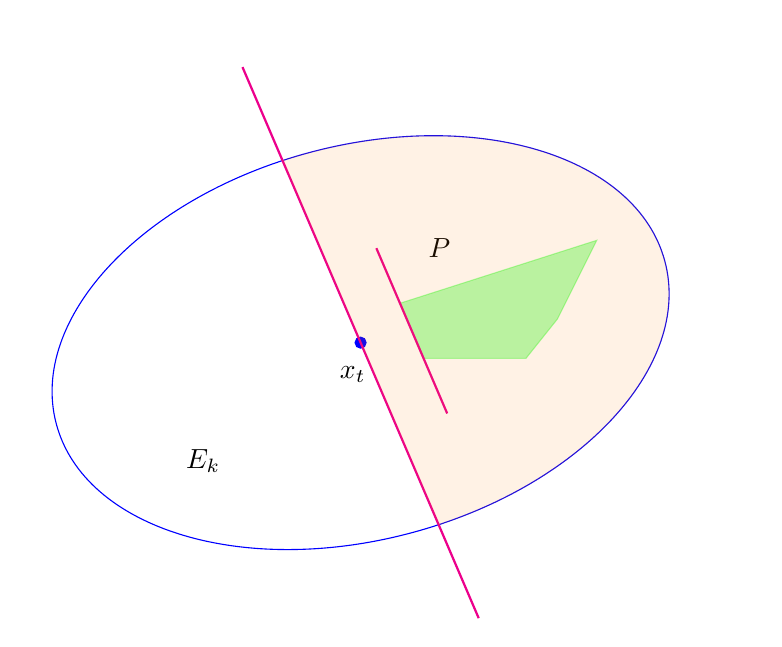
\begin{tikzpicture}
\node[] () at (-2,-1.5) {\(E_{k}\)};
\draw[blue, rotate=15] (0,0) ellipse [x radius=4cm, y radius=2.5cm];
\draw[blue, fill] (0,0) circle [radius=0.7mm];
\node[] () at (-0.1,-0.4) {\(\vect{x}_t\)};
\draw[green, fill, opacity=0.3] (0.5,0.5) -- (3,1.3) -- (2.5,0.3) --
(2.1,-0.2) -- (0.8,-0.2) -- cycle;
\node[] () at (1,1.2) {\(P\)};
\draw[magenta, thick] (0.2,1.2) -- (1.1,-0.8996);
\draw[magenta, thick] (-1.5,3.4995) -- (1.5,-3.4995);
\begin{scope}
\clip[] (-1, 2.3333) -- (1,-2.3333) -- (5,-2.3333) -- (5,4) -- cycle;
\draw[fill, orange, opacity=0.1, rotate=15] (0,0) ellipse [x radius=4cm, y radius=2.5cm];
\end{scope}
\end{tikzpicture}
\end{center}
Then, it turns out to be possible to find a new ellipsoid \(E_{t+1}\) that
covers the half-ellipsoid, with volume being only a fraction of that of the
previous ellipsoid \(E_t\):
\begin{center}
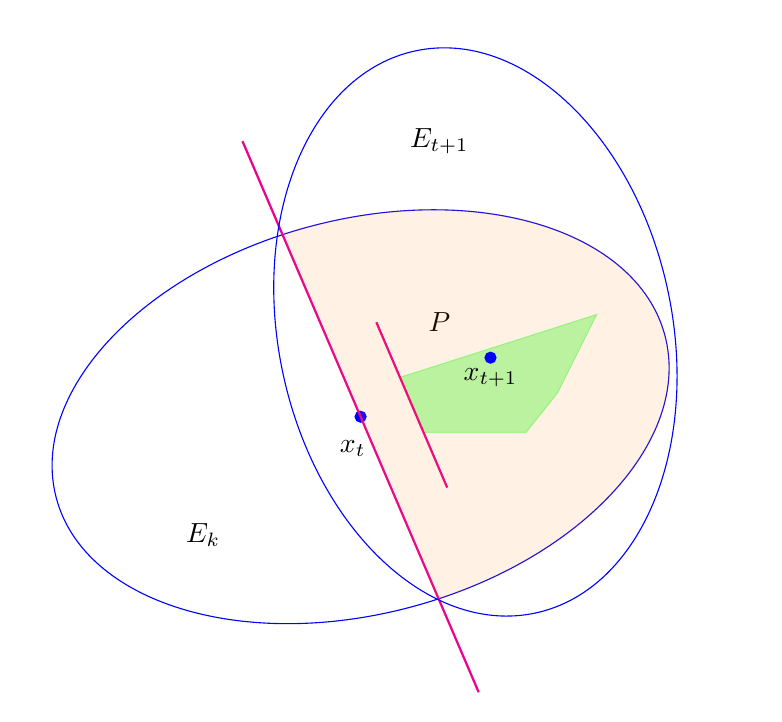
\begin{tikzpicture}
\node[] () at (-2,-1.5) {\(E_{k}\)};
\draw[blue, rotate=15] (0,0) ellipse [x radius=4cm, y radius=2.5cm];
\draw[blue, fill] (0,0) circle [radius=0.7mm];
\node[] () at (-0.1,-0.4) {\(\vect{x}_t\)};
\draw[green, fill, opacity=0.3] (0.5,0.5) -- (3,1.3) -- (2.5,0.3) --
(2.1,-0.2) -- (0.8,-0.2) -- cycle;
\node[] () at (1,1.2) {\(P\)};
\draw[magenta, thick] (0.2,1.2) -- (1.1,-0.8996);
\draw[magenta, thick] (-1.5,3.4995) -- (1.5,-3.4995);
\begin{scope}
\clip[] (-1, 2.3333) -- (1,-2.3333) -- (5,-2.3333) -- (5,4) -- cycle;
\draw[fill, orange, opacity=0.1, rotate=15] (0,0) ellipse [x radius=4cm, y radius=2.5cm];
\end{scope}
\draw[blue, rotate=102] (0.75,-1.65) ellipse [x radius=3.65cm, y radius=2.5cm];
\node[] () at (1,3.5) {\(E_{t+1}\)};
\draw[blue, fill] (1.65,0.75) circle [radius=0.7mm];
\node[] () at (1.65,0.5) {\(\vect{x}_{t+1}\)};
\end{tikzpicture}
\end{center}
\end{enumerate}
As the ellipsoids obtained in this way have shrinking volumes, eventually we
would either find a point in \(P\) or find that the volume of \(P\) is so small
that it must be empty (more details will be discussed in
\labelcref{it:ellip-method-implement}). In either way, the linear feasibility
problem is solved. This gives us an intuitive idea on how the ellipsoid method
works.

Next, we will prove mathematical results that justify the ellipsoid method.
\item \textbf{Construction of those ellipsoids.} The first result to be
established is an explicit way of constructing the ellipsoids that satisfy the
aforementioned properties. Particularly, we will provide a formula that computes
the next ellipsoid \(E_{t+1}\) given the ellipsoid \(E_{k}\).

\begin{theorem}[Formula for ``next ellipsoid'']
\label{thm:next-ellipsoid-fmla}
Let \(n\ge 2\), \(E=E(\vect{z},D)\) be an ellipsoid in \(\R^n\), and
\(\vect{a}\in\R^n\) be nonzero. Consider the halfspace
\(H:=\{\vect{x}\in\R^n:\vect{a}^{T}\vect{x}\ge\vect{a}^{T}\vect{z}\}\). Let
\[
\bar{\vect{z}}=\vect{z}+\frac{1}{n+1}\cdot \frac{D\vect{a}}{\sqrt{\vect{a}^{T}D\vect{a}}}
\quad\text{and}\quad
\bar{D}=\frac{n^{2}}{n^{2}-1}\left(D-\frac{2}{n+1}\cdot 
\frac{D\vect{a}\vect{a}^{T}D}{\vect{a}^{T}D\vect{a}}\right).
\]
Then \(\bar{D}\) is positive definite and hence
\(E':=E(\bar{\vect{z}},\bar{D})\) is an ellipsoid. Furthermore, we have \(E\cap
H\subseteq E'\) \emph{(containing the half-ellipsoid)} and
\(\vol{E'}<e^{-\frac{1}{2(n+1)}}\vol{E}\) \emph{(smaller volume)}.
\end{theorem}
\begin{note}
In the special case where \(E\) is the unit ball (i.e.,
\(\vect{z}=\vect{0}\) and \(D=I\)) with
\(\vect{a}=\vect{e}_1=(1,0,\dotsc,0)\), we would have
\(H=\{\vect{x}\in\R^n:x_1\ge 0\}\),
\[
\bar{\vect{z}}=\frac{1}{n+1}\cdot \vect{e}_1
\quad\text{and}\quad
\bar{D}=\frac{n^{2}}{n^{2}-1}\left(I-\frac{2}{n+1}\cdot \vect{e}_1\vect{e}_1^{T}\right).
\]
\end{note}

\begin{pf}
Here we only prove the special case where \(E\) is the unit ball (i.e.,
\(\vect{z}=\vect{0}\) and \(D=I\)) with
\(\vect{a}=\vect{e}_1=(1,0,\dotsc,0)\). With the special case proved, the
general case follows by performing suitable affine transformations; see
\textcite[Theorem~8.1]{bertsimas1997introduction} for more details.

\textbf{Showing the positive definiteness of \(\bar{D}\).}
Note that
\[
\bar{D}=\frac{n^{2}}{n^{2}-1}\left(
\begin{bmatrix}1&0&\cdots&0\\
0&1&\cdots&0\\
\vdots&\vdots&\ddots&\vdots \\
0&0&\cdots&1\\
\end{bmatrix}
-\frac{2}{n+1}
\begin{bmatrix}1&0&\cdots&0\\
0&0&\cdots&0\\
\vdots&\vdots&\ddots&\vdots \\
0&0&\cdots&0\\
\end{bmatrix}\right)
=\frac{n^{2}}{n^{2}-1}
\begin{bmatrix}\frac{n-1}{n+1}&0&\cdots&0\\
0&1&\cdots&0\\
\vdots&\vdots&\ddots&\vdots \\
0&0&\cdots&1\\
\end{bmatrix}.
\]
Hence, for all \(\vect{x}\ne\vect{0}\), we have
\[
\vect{x}^{T}\bar{D}\vect{x}=\frac{n^{2}}{n-1}\left(\frac{n-1}{n+1}x_1^{2}
+\sum_{i=2}^{n}x_i^{2}\right)
\overset{\text{(\(x_i\ne 0\) for some \(i\))}}{>}0.
\]
\textbf{Showing that \(E\cap H\subseteq E'\).}
Since \(\bar{D}\) is a diagonal matrix, we can compute its inverse conveniently:
\[
\bar{D}^{-1}=\frac{n^{2}-1}{n^{2}}
\begin{bmatrix}\frac{n+1}{n-1}&0&\cdots&0\\
0&1&\cdots&0\\
\vdots&\vdots&\ddots&\vdots \\
0&0&\cdots&1\\
\end{bmatrix}
=\begin{bmatrix}\frac{(n+1)^{2}}{n^{2}}&0&\cdots&0\\
0&\frac{n^{2}-1}{n^{2}}&\cdots&0\\
\vdots&\vdots&\ddots&\vdots \\
0&0&\cdots&\frac{n^{2}-1}{n^{2}}\\
\end{bmatrix}.
\]
Hence, we have
\begin{align*}
E'&=\{\vect{x}\in\R^n: (\vect{x}-\vect{z})^{T}\bar{D}^{-1}(\vect{x}-\vect{z})\le 1\} \\
&=\left\{\vect{x}\in\R^n: \frac{(n+1)^{2}}{n^{2}}\left(x_1-\frac{1}{n+1}\right)^{2}
+\frac{n^{2}-1}{n^{2}}\sum_{i=2}^{n}x_i^{2}\le 1\right\} \\
&=\left\{\vect{x}\in\R^n: \vc{\frac{(n+1)^{2}}{n^{2}}x_1^{2}}-\frac{2(n+1)}{n^{2}}x_1
+\frac{1}{n^{2}}+\vc{\frac{n^{2}-1}{n^{2}}\sum_{i=2}^{n}x_i^{2}}\le 1\right\} \\
&=\left\{\vect{x}\in\R^n: \vc{\frac{n^{2}-1}{n^{2}}\sum_{i=1}^{n}x_i^{2}
+\frac{(n+1)^{2}-(n^{2}-1)}{n^{2}}x_1^{2}}
-\frac{2(n+1)}{n^{2}}x_1
+\frac{1}{n^{2}}\le 1\right\} \\
&=\left\{\vect{x}\in\R^n: \frac{n^{2}-1}{n^{2}}\sum_{i=1}^{n}x_i^{2}
+\frac{2(n+1)}{n^{2}}x_1(x_1-1)
+\frac{1}{n^{2}}\le 1\right\}.
\end{align*}
For all \(\vect{x}\in E\cap H\), we have \(\sum_{i=1}^{n}x_i^{2}\le 1\) and
\(x_1\ge 0\), and thus
\[
\frac{n^{2}-1}{n^{2}}\underbrace{\sum_{i=1}^{n}x_i^{2}}_{\le 1}
+\frac{2(n+1)}{n^{2}}x_1(x_1-1)
+\frac{1}{n^{2}}
\le \frac{2(n+1)}{n^{2}}\underbrace{x_1}_{\ge 0}(\underbrace{x_1-1}_{\le 0})+1
\le 1,
\]
meaning that \(\vect{x}\in E'\).

\textbf{Showing that \(\vol{E'}<e^{-\frac{1}{2(n+1)}}\vol{E}\).}
By \labelcref{it:ellip-method-geo-prop}, since \(E\) is the unit ball we know
\(\vol{E'} =\det \bar{D}^{1/2}\vol{E}=\sqrt{\det \bar{D}}\vol{E}\). Therefore,
it suffices to show that \(\sqrt{\det \bar{D}}<e^{-\frac{1}{2(n+1)}}\).

To show this, consider
\begin{align*}
\det\bar{D}&=\det\left(\frac{n^{2}}{n^{2}-1}
\begin{bmatrix}\frac{n-1}{n+1}&0&\cdots&0\\
0&1&\cdots&0\\
\vdots&\vdots&\ddots&\vdots \\
0&0&\cdots&1\\
\end{bmatrix}\right)
=\left(\frac{n^{2}}{n^{2}-1}\right)^{n}\det
\begin{bmatrix}\frac{n-1}{n+1}&0&\cdots&0\\
0&1&\cdots&0\\
\vdots&\vdots&\ddots&\vdots \\
0&0&\cdots&1\\
\end{bmatrix} \\
&=\left(\frac{n^{2}}{n^{2}-1}\right)^{n}\frac{n-1}{n+1}
=\left(\frac{n^{2}}{n^{2}-1}\right)^{n-1}\frac{n^{2}}{n^{2}-1}\frac{n-1}{n+1}
=\left(1+\frac{1}{n^{2}-1}\right)^{n-1}\frac{n^{2}}{(n+1)^{2}} \\
&=\left(1+\frac{1}{n^{2}-1}\right)^{n-1}\left(1-\frac{1}{n+1}\right)^{2}
\overset{(1+x\le e^{x})}{\le}
\left(e^{\frac{1}{n^{2}-1}}\right)^{n-1}\left(e^{-\frac{1}{n+1}}\right)^{2}
=e^{-\frac{1}{n+1}}.
\end{align*}
Hence, we have \(\sqrt{\det \bar{D}}\le e^{-\frac{1}{2(n+1)}}\).
\end{pf}
\item \label{it:ellip-method-implement} \textbf{Implementation of the ellipsoid
method.} Based on \Cref{thm:next-ellipsoid-fmla}, we can implement the
ellipsoid method for solving the linear feasibility problem. But here we need
to impose some assumptions on the polyhedron \(P\): (i) \(P\) is bounded, and
(ii) \(P\) is either empty or \defn{full-dimensional} (i.e., it has positive
volume).
\begin{note}
It is possible to have a nonempty polyhedron with zero volume, e.g., a line in
\(\R^3\), but such polyhedron would have a lower dimension than the space. This
explains the name ``full-dimensional''.
\end{note}

With \(P\) being bounded, we know \(P\subseteq E(\vect{x}_0,r^{2}I)\) for some
\(\vect{x}_0\in P\) and sufficiently large \(r>0\). Hence, we can set
\(V:=\vol{E(\vect{x}_0,r^{2}I)}\) to serve as an initial upper bound on
\(\vol{P}\).  Also, in case \(P\) is full-dimensional, we would have
\(\vol{P}>0\), and thus \(\vol{P}\ge v\) for some \(v>0\). Altogether, we would
have \(v\le \vol{P}\le V\).

Knowing \(\vect{x}_0\), \(r\), \(v\), and \(V\), the ellipsoid method can then
be implemented as follows.
\begin{enumerate}[label={(\arabic*)}]
\item \emph{(initialization)}
\begin{itemize}
\item \(t^{*}\leftarrow\lceil 2(n+1)\ln(V/v)\rceil\).
\item \(E_0\leftarrow E(\vect{x}_0,r^{2}I)\).
\item \(D_0\leftarrow r^{2}I\).
\item \(t\leftarrow 0\).
\end{itemize}
\item \emph{(main iteration)} Repeat the following steps until termination.
\begin{enumerate}
\item If \(t=t^{*}\), conclude that \(P\) is empty and stop \faIcon[regular]{pause-circle}.
\item If \(\vect{x}_t\in P\), conclude that \(P\) is nonempty and stop
\faIcon[regular]{pause-circle}.
\item If \(\vect{x}_t\notin P\), find a violated constraint with
\(\vect{a}_i^{T}\vect{x}_t<b_i\).
\item Let
\(H_t:=\{\vect{x}\in\R^n:\vect{a}_i^{T}\vect{x}\ge\vect{a}_i^{T}\vect{x}_t\}\).
Construct the next ellipsoid \(E_{t+1}\) that contains \(E_t\cap H_t\) and has
a smaller volume than \(E_t\) as in \Cref{thm:next-ellipsoid-fmla}:
\begin{align*}
\vect{x}_{t+1}&\leftarrow\vect{x}_{t}+\frac{1}{n+1}
\cdot \frac{D_t\vect{a}_i}{\sqrt{\vect{a}_i^{T}D_t\vect{a}_i}}, \\
D_{t+1}&\leftarrow\frac{n^{2}}{n^{2}-1}\left(D_t-\frac{2}{n+1}\cdot 
\frac{D_t\vect{a}_i\vect{a}_i^{T}D_t}{\vect{a}_i^{T}D_t\vect{a}_i}\right).
\end{align*}
\item \(t\leftarrow t+1\).
\end{enumerate}
\end{enumerate}
\begin{remark}
\item The case where \(t=t^{*}\) corresponds to the conclusion that ``the volume of
\(P\) is so small that it must be empty'' mentioned in the intuitive idea.  See
the proof of \Cref{thm:ellip-method-correct} for more details about this.
\item By induction, we can show that \(P\subseteq E_t\) for every \(t\) in the
ellipsoid method.

First, by construction we have \(P\subseteq E_0\). Next, assume \(P\subseteq
E_k\) for some \(k<t^{*}\). The existence of \(E_k\) implies that there is a
violated constraint \(\vect{a}_{i}^{T}\vect{x}_{k}< b_{i}\). Then, for all
\(\vect{x}\in P\), we have \(\vect{a}_{i}^{T}\vect{x}\ge
b_{i}>\vect{a}_{i}^{T}\vect{x}_{k}\), implying that \(P\subseteq H_k\), and
hence \(P\subseteq E_k\cap H_k
\overset{\text{(\Cref{thm:next-ellipsoid-fmla})}}{\subseteq} E_{k+1}\). This
completes the proof by induction.
\end{remark}
\item \textbf{Correctness of the ellipsoid method.} From the implementation of
the ellipsoid method in \labelcref{it:ellip-method-implement}, while we know
that it must terminate with a conclusion that \(P\) is empty/nonempty by
construction, we actually have not shown that such conclusion is \emph{correct}.
Particularly, it may be possible that when \(t=t^{*}\), we conclude that \(P\) is
empty but it is indeed not. \begin{note}
On the other hand, it is not possible to wrongly conclude that \(P\) is nonempty,
since \(\vect{x}_t\in P\) does imply that \(P\) is nonempty.
\end{note}

To fully justify the ellipsoid method, we need the following result that
guarantees its correctness.

\begin{theorem}[The ellipsoid method is correct]
\label{thm:ellip-method-correct}
Let \(P\) be a bounded polyhedron that is either empty or full-dimensional.
The ellipsoid method from \labelcref{it:ellip-method-implement} correctly
determines whether \(P\) is empty, i.e., if \(\vect{x}_{t}\notin P\) for all
\(t=0,1,\dotsc,t^{*}-1\) (so we would stop at the case where \(t=t^{*}\)), then
\(P\) is empty.
\end{theorem}
\begin{pf}
Suppose \(\vect{x}_{t}\notin P\) for all \(t=0,1,\dotsc,t^{*}-1\). Then, by
\Cref{thm:next-ellipsoid-fmla} we have
\[
\vol{E_{t^{*}}}<e^{-\frac{t^{*}}{2(n+1)}}\vol{E_0}
\le Ve^{-\frac{2(n+1)\ln (V/v)}{2(n+1)}}
=V\cdot \frac{v}{V}=v.
\]
Since \(P\subseteq E_{t^{*}}\), we have \(\vol{P}\le\vol{E_{t^{*}}}<v\), which
implies that \(P\) is not full-dimensional, and hence empty.
\end{pf}
\item \textbf{Relaxing the assumptions on the boundedness and full-dimensionality.}
In the ellipsoid method, we require the boundedness and full-dimensionality
assumptions, but in practice the polyhedron \(P\) in consideration may violate 
one of these assumptions. In view of this, here we will discuss a method that
allows such assumptions to be relaxed, but requires us to further assume that
all the entries of \(A\) and \(\vect{b}\) for the polyhedron \(P\) are integers
\emph{(integer data)}.

The basic idea of the method is as follows. Given any polyhedron \(P\)
(possibly violating the assumptions on boundedness and full-dimensionality), we
can construct another polyhedron \(P'\) such that (i) \(P\) is nonempty iff
\(P'\) is nonempty (so we can check whether \(P'\) is empty rather than \(P\)),
and (ii) if \(P'\) is nonempty, then \(v\le \vol{P'}\le V\) for some \(v,V>0\);
here, the upper and lower bounds on \(\vol{P'}\) correspond to the boundedness
and full-dimensionality assumptions respectively. Then, we can apply the
ellipsoid method on \(P'\) to deduce whether \(P\) is empty.

\item\label{it:relax-bdd-assum} \textbf{Relaxing the boundedness assumption.}
To relax the boundedness assumption, we need to establish a result that bounds
every vertex of the polyhedron \(P\) with integer data.

\begin{proposition}
\label{prp:polyhedron-vertex-bdd}
Let \(A\in \Z^{m\times n}\), \(\vect{b}\in\Z^{m}\), and \(U\in\N\) be an upper
bound on the absolute values of the entries in \(A\) and
\(\vect{b}\).\footnote{Such \(U\) always exists as there are only finitely many
entries here.} Suppose that the polyhedron \(P\) in consideration has a vertex.
\begin{enumerate}
\item \emph{(general form)} Every vertex \(\vect{x}=(x_1,\dotsc,x_n)\) of the polyhedron
\(P=\{\vect{x}\in\R^n:A\vect{x}\ge\vect{b}\}\) satisfies \(|x_j|\le (nU)^{n}\)
for every \(j=1,\dotsc,n\).
\item \emph{(standard form)} Every vertex \(\vect{x}=(x_1,\dotsc,x_n)\) of the polyhedron
\(P=\{\vect{x}\in\R^n:A\vect{x}=\vect{b}, \vect{x}\ge\vect{0}\}\) satisfies
\(|x_j|\le (mU)^{m}\) for every \(j=1,\dotsc,n\).
\end{enumerate}
\end{proposition}
\begin{pf}
\begin{enumerate}
\item Fix any vertex \(\vect{x}\) of \(P\). Since \(\vect{x}\) is also a basic
feasible solution of \(P\), we can choose \(n\) linearly independent active
constraints at \(\vect{x}\), and then write
\(\widehat{A}\vect{x}=\widehat{\vect{b}}\), where \(\widehat{A}\) is an
\(n\times n\) invertible submatrix of \(A\) and \(\widehat{\vect{b}}\) is the
corresponding \(n\)-dimensional subvector of \(\vect{b}\). By Cramer's rule,
the solution \(\vect{x}\) to \(\widehat{A}\vect{x}=\widehat{\vect{b}}\) is given by
\(x_j=\det\widehat{A}^{j}/\det\widehat{A}\) for all \(j=1,\dotsc,n\), where
\(\widehat{A}^{j}\) denotes the matrix \(\widehat{A}\) with its \(j\)th column
replaced by \(\widehat{\vect{b}}\).

Using the Leibniz formula for determinants, we have
\(\det\widehat{A}^{j}=\sum_{\sigma}^{}(-1)^{|\sigma|}
\prod_{i=1}^{n}\widetilde{a}_{i,\sigma(i)}\), where the summation is over all
the \(n!\) permutations \(\sigma=(\sigma(1),\dotsc,\sigma(n))\) of
\(\{1,\dotsc,n\}\), with \(\widetilde{a}_{ij}=\widehat{b}_j\) and
\(\widetilde{a}_{ik}=\widehat{a}_{ik}\) for all \(k\ne j\); here \(|\sigma|\)
denotes the number of \emph{inversions} of the permutation \(\sigma\), i.e., number
of times where \(i<j\) while \(\sigma(i)>\sigma(j)\).

Then, consider
\begin{align*}
|\det \widehat{A}^{j}|
&=\left|\sum_{\sigma}^{}(-1)^{|\sigma|}
\prod_{i=1}^{n}\widetilde{a}_{i,\sigma(i)}\right|
\overset{\text{(triangle)}}{\le}
\sum_{\sigma}^{}\prod_{i=1}^{n}|\widetilde{a}_{i,\sigma(i)}| \\
\overset{(|\widetilde{a}_{i,\sigma(i)}|\le U)}&{\le}\sum_{\sigma}^{}U^{n}
=n!U^n\overset{(n!=n(n-1)\dotsb 1\le n(n)\dotsb n=n^n)}{\le} \vc{(nU)^n}
\end{align*}
for all \(j=1,\dotsc,n\). Furthermore, since \(\det\widehat{A}\ne 0\) (as
\(\widehat{A}\) is invertible) and \(\widehat{A}\) has integer entries, we must
have \(|\det\widehat{A}|\ge \orc{1}\). Hence, for all \(j=1,\dotsc,n\), we have
\(|x_j|=|\det\widehat{A}^{j}|/|\det\widehat{A}|\le \vc{(nU)^{n}}/\orc{1}=(nU)^{n}\).
\item Use the same argument as in (a) but replace the \(n\times n\) matrix
\(\widehat{A}\) by the basis matrix \(B\). In case \(A\) has linearly
independent rows, the basis matrix would be of size \(m\times m\). Otherwise,
we can remove redundant rows of \(A\) and so the size of the basis matrix would
be smaller than \(m\times m\). Thus, in either case, repeating the argument in
(a) would at least yield the bound \(|x_j|\le (mU)^{m}\) for every
\(j=1,\dotsc,n\).
\end{enumerate}
\end{pf}

To use \Cref{prp:polyhedron-vertex-bdd} for relaxing the boundedness
assumption, we can do the following. First we start with any polyhedron
\(P=\{\vect{x}\in\R^n:A\vect{x}\ge\vect{b}\}\), where the rows of \(A\) span
\(\R^n\) (implying that \(m\ge n\)). Then, define
\[
P_{B}:=\{\vect{x}\in P:|x_j|\le (nU)^{n}~\forall j=1,\dotsc,n\}.
\]
Here, the polyhedron \(P_{B}\) satisfies the following properties:
\begin{enumerate}
\item \(P\) is nonempty iff \(P_{B}\) is nonempty.

\begin{note}
This holds under the assumption that the rows of \(A\) span \(\R^n\), which
would mean that \(P\) is nonempty iff \(P\) has a vertex iff \(P_{B}\) is
nonempty.
\end{note}
\item \(P_{B}\) is a bounded polyhedron contained in the ball
\(E_0:=E(\vect{0},r^{2}I):=E(\vect{0},n(nU)^{2n}I)\).

\begin{note}
The volume of \(E_0\) is less than
\((2r)^{n}=(2n(nU)^{n})^{n}=(2n)^{n}(nU)^{n^{2}}\), so we can take
\(V=(2n)^{n}(nU)^{n^{2}}\) as the initial upper bound of \(\vol{P_B}\) in the
ellipsoid method.
\end{note}
\end{enumerate}
\item \label{it:relax-full-d-assum} \textbf{Relaxing the full-dimensionality assumption.}
Next, we will discuss how the full-dimensionality assumption can be relaxed.
Similar to \labelcref{it:relax-bdd-assum}, a result is needed for constructing
a polyhedron that is full-dimensional from a polyhedron \(P\). The key idea of
this result is that a small perturbation of a nonempty polyhedron \(P\)
(possibly not full-dimensional) can yield a full-dimensional polyhedron
\(P_{\varepsilon}\).
\begin{center}
\begin{tikzpicture}
\draw[blue] (0,0) -- (4,1);
\draw[blue] (1,2) -- (4,-1.5);
\draw[blue] (-0.5,1.5) -- (5,-0.4);
\draw[orange, fill] (2.25,0.55) circle [radius=0.6mm];
\end{tikzpicture}
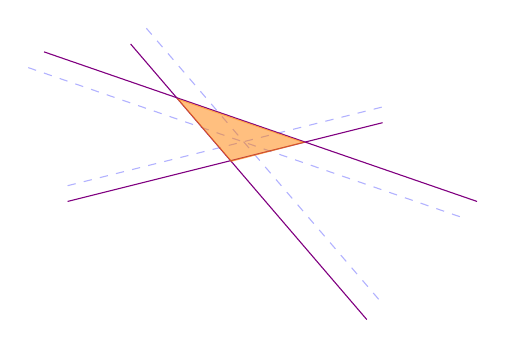
\begin{tikzpicture}
\draw[blue, opacity=0.3, dashed] (0,0) -- (4,1);
\draw[blue, opacity=0.3, dashed] (1,2) -- (4,-1.5);
\draw[blue, opacity=0.3, dashed] (-0.5,1.5) -- (5,-0.4);
\draw[violet] (0,-0.2) -- (4,0.8);
\draw[violet] (0.8,1.8) -- (3.8,-1.7);
\draw[violet] (-0.3,1.7) -- (5.2,-0.2);
\draw[orange, fill, opacity=0.5] (2.08,0.31) -- (1.4,1.1) -- (3,0.55) -- cycle;
\end{tikzpicture}
\end{center}
\begin{proposition}
\label{prp:nonempty-small-perturb-full-d}
Let \(P=\{\vect{x}\in\R^n:A\vect{x}\ge\vect{b}\}\) be a polyhedron with
\(A\in\Z^{m\times n}\), \(\vect{b}\in \Z^{m}\), and \(U\in\N\) being an upper
bound on the absolute values of the entries in \(A\) and
\(\vect{b}\). We let
\[
\varepsilon=\frac{1}{2(n+1)}((n+1)U)^{-(n+1)}\quad\text{and}\quad
P_{\varepsilon}=\{\vect{x}\in\R^n:A\vect{x}\ge\vect{b}-\varepsilon\vect{1}\}
\]
where \(\vect{1}=(1,\dotsc,1)\in\R^m\).
\begin{enumerate}
\item If \(P\) is empty, then \(P_{\varepsilon}\) is empty.
\item If \(P\) is nonempty, then \(P_{\varepsilon}\) is full-dimensional.
\end{enumerate}
\end{proposition}
\begin{pf}
\begin{enumerate}
\item Assume \(P\) is empty.

\textbf{Setting up two pairs of primal and dual.} Then consider the following infeasible
(primal) LP problem:
\begin{align*}
\text{min}\quad&\vect{0}^{T}\vect{x} \\
\text{s.t.}\quad&A\vect{x}\ge\vect{b}
\end{align*}
and its dual:
\begin{align*}
\text{max}\quad&\vect{b}^{T}\vect{y} \\
\text{s.t.}\quad&A^{T}\vect{y}=\vect{0} \\
&\vect{y}\ge\vect{0}.
\end{align*}
Since the primal problem is infeasible, by \labelcref{it:primal-dual-poss} we
know that either the dual problem is infeasible or its optimal value is \(\infty\).
Observing that \(\vect{y}=\vect{0}\) is a feasible solution to the dual, we
deduce that its optimal value must be \(\infty\). So particularly, there exists
\(\vect{y}\in\R^m\) such that \(A^{T}\vect{y}=\vect{0}\) and
\(\vect{b}^{T}\vect{y}=1\).

Also, consider the ``perturbed'' primal:
\begin{align*}
\text{min}\quad&\vect{0}^{T}\vect{x} \\
\text{s.t.}\quad&A\vect{x}\ge\vect{b}-\varepsilon\vect{1},
\end{align*}
and the ``perturbed'' dual:
\begin{align*}
\text{max}\quad&(\vect{b}-\varepsilon\vect{1})^{T}\vect{y} \\
\text{s.t.}\quad&A^{T}\vect{y}=\vect{0} \\
&\vect{y}\ge\vect{0}.
\end{align*}

\textbf{Showing the existence of feasible solution to the ``perturbed'' dual
with positive objective function value.}
Let \(P_1=\{\vect{y}\in\R^m:A^{T}\vect{y}=\vect{0},
\vect{b}^{T}\vect{y}=1, \vect{y}\ge\vect{0}\}\), which is a nonempty standard
form polyhedron.  By \Cref{cor:std-form-has-vertex}, \(P_1\) has a vertex and
hence by \Cref{prp:polyhedron-vertex-bdd}, there exists a basic feasible
solution \(\widehat{\vect{y}}\) of \(P_1\) such that \(|\widehat{y_j}|\le
((n+1)U)^{n+1}~\forall j=1,\dotsc,m\) (the ``\(m\)'' for that result is \(n+1\)
here). Since \(\widehat{\vect{y}}\) is a basic feasible solution, at most
\(n+1\) of its components are nonzero, and thus
\(\vect{1}^{T}\widehat{\vect{y}}=\sum_{j=1}^{m}\widehat{y}_j\le (n+1)((n+1)U)^{n+1}\).
This implies that
\[
(\vect{b}-\varepsilon\vect{1})^{T}\widehat{\vect{y}}
=\vect{b}^{T}\widehat{\vect{y}}-\varepsilon\vect{1}^{T}\vect{y}
\ge 1-\frac{1}{2(n+1)}((n+1)U)^{-(n+1)}(n+1)((n+1)U)^{n+1}
=1-\frac{1}{2}>0,
\]
and hence such \(\widehat{\vect{y}}\) is a feasible solution to the
``perturbed'' dual with positive objective function value.

\textbf{Completing the proof by showing that the optimal value of ``perturbed''
dual is \(\infty\).}
Fix any \(\lambda>0\). Since \(A^{T}(\lambda\widehat{\vect{y}})=\vect{0}\) and
\(\lambda\widehat{\vect{y}}\ge\vect{0}\), \(\lambda\widehat{\vect{y}}\) is a
feasible solution to the ``perturbed'' dual. Now, note that the objective function
at \(\lambda\widehat{\vect{y}}\) is
\((\vect{b}-\varepsilon\vect{1})^{T}(\lambda\widehat{\vect{y}})
=\lambda\underbrace{(\vect{b}-\varepsilon\vect{1})^{T}\widehat{\vect{y}}}_{>0}\)
, which can be arbitrarily large as \(\lambda\) is increased, so we conclude
that the optimal value of ``perturbed'' dual is \(\infty\).
Hence, by \labelcref{it:primal-dual-poss}, we know that the ``perturbed''
primal must be infeasible, implying that \(P_{\varepsilon}\) is empty.
\item Assume \(P\) is nonempty and let \(\vect{x}\in P\), which satisfies that
\(A\vect{x}\ge\vect{b}\). Let \(C:=\{\vect{z}\in\R^n:|z_j-x_j|\le
\varepsilon/(nU)~\forall j=1,\dotsc,n\}\), which is a cube with positive volume.

Fix any \(\vect{z}\in C\). Note that we have for all \(i=1,\dotsc,m\),
\[
\vect{a}_i^{T}\vect{z}
=\vect{a}_{i}^{T}\vect{x}+\underbrace{\vect{a}_{i}^{T}(\vect{z}-\vect{x})}_{
\sum_{j=1}^{n}a_{ij}(z_j-x_j)}
\ge b_i-\sum_{j=1}^{n}|a_{ij}|\cdot |z_j-x_j|
\ge b_i-\sum_{j=1}^{n}U\cdot \varepsilon/(nU)
=b_i-\varepsilon,
\]
which implies that \(\vect{z}\in P_{\varepsilon}\). Hence, \(C\subseteq P_{\varepsilon}\),
and thus \(\vol{P_{\varepsilon}}\ge\vol{C}>0\), meaning that
\(P_{\varepsilon}\) is full-dimensional.
\end{enumerate}
\end{pf}

From \Cref{prp:nonempty-small-perturb-full-d}, we know that the perturbed
polyhedron \(P_{\varepsilon}\) satisfies:
\begin{enumerate}
\item \(P\) is nonempty iff \(P_{\varepsilon}\) is nonempty.
\item \(P_{\varepsilon}\) is either empty or full-dimensional (as \(P\) is
either empty or nonempty).
\end{enumerate}
Therefore, it can be used to relax the full-dimensionality assumption.
Furthermore, we can apply the method from \labelcref{it:relax-bdd-assum} to
obtain a bounded and full-dimensional polyhedron that is nonempty iff the
original polyhedron is nonempty (more details in
\labelcref{it:ellip-method-poly-time}).
However, to perform the ellipsoid method on such polyhedron, we would need the
input \(v\), which is not given in \Cref{prp:nonempty-small-perturb-full-d}.
The following result addresses this need and provides a possible value of
\(v\).

\begin{proposition}
\label{prp:bdd-full-d-polyhedron-v}
Let \(A\in\Z^{m\times n}\), \(\vect{b}\in \Z^{m}\), and \(U\in\N\) be an upper
bound on the absolute values of the entries in \(A\) and \(\vect{b}\). Let
\(P=\{\vect{x}\in\R^n:A\vect{x}\ge\vect{b}\}\) be a bounded and
full-dimensional polyhedron. We have
\[
\vol{P}>n^{-n}(nU)^{-n^{2}(n+1)}
\]
(hence one possible choice of \(v\) is \(n^{-n}(nU)^{-n^{2}(n+1)}\)).
\end{proposition}
\begin{pf}
Here, we will use the fact that a nonempty and bounded polyhedron is the
\emph{convex hull} of its vertices \(\vect{v}^{0},\dotsc,\vect{v}^{N}\), given
by \(\conv{\{\vect{v}^{0},\dotsc,\vect{v}^{N}\}}
:=\{\sum_{i=0}^{N}\lambda_{i}\vect{v}^{i}:\sum_{i=0}^{N}\lambda_k=1,
\lambda_i\ge 0~\forall i\}\).

With \(P\) being full-dimensional, it can be shown that there are \(n+1\)
vertices of \(P\) that are not on a common hyperplane, say
\(\vect{v}^{0},\dotsc,\vect{v}^{n}\) without loss of generality. Now, we let
\(Q=\conv{\{\vect{v}^{0},\dotsc,\vect{v}^{n}\}}\subseteq P\), 
and let \(\Delta_n^c:=\{\vect{x}\in\R^n:\sum_{i=1}^{n}x_i\le 1, x_i\ge
0~\forall i\}\) be a \emph{corner of cube} for each \(n\in\N\), whose volume
can be shown to be \(1/n!\).
\begin{center}
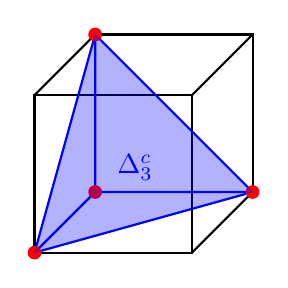
\begin{tikzpicture}
\coordinate (A) at (0, 0, 0);
\coordinate (B) at (2, 0, 0);
\coordinate (C) at (2, 2, 0);
\coordinate (D) at (0, 2, 0);
\coordinate (E) at (0, 0, 2);
\coordinate (F) at (2, 0, 2);
\coordinate (G) at (2, 2, 2);
\coordinate (H) at (0, 2, 2);
\coordinate (S1) at (0, 0, 0);
\coordinate (S2) at (2, 0, 0);
\coordinate (S3) at (0, 2, 0);
\coordinate (S4) at (0, 0, 2);

\draw[thick] (A) -- (B) -- (C) -- (D) -- cycle;
\draw[thick] (E) -- (F) -- (G) -- (H) -- cycle;
\draw[thick] (A) -- (E);
\draw[thick] (B) -- (F);
\draw[thick] (C) -- (G);
\draw[thick] (D) -- (H);
\draw[thick, blue] (S1) -- (S2) -- (S3) -- cycle;
\draw[thick, blue] (S1) -- (S4);
\draw[thick, blue] (S2) -- (S4);
\draw[thick, blue] (S3) -- (S4);
\draw[red, fill] (S1) circle [radius=0.8mm];
\draw[red, fill] (S2) circle [radius=0.8mm];
\draw[red, fill] (S3) circle [radius=0.8mm];
\draw[red, fill] (S4) circle [radius=0.8mm];
\draw[blue, fill, opacity=0.3] (S2) -- (S3) -- (S4) -- cycle;
\node[blue] () at (0.7, 0.5, 0.5) {\(\Delta_{3}^{c}\)};
\end{tikzpicture}
\end{center}
Next, we will use the fact that \(Q\) can be obtained by applying an affine
transformation \(S\) on \(\Delta_{n}^{c}\), with \(S\) characterized by the
mappings for vertices: \(S(\vect{e}_i)=\vect{v}^{i}\) for all \(i=0,\dotsc,n\),
where \(\vect{e}_0:=\vect{0}\).
\begin{center}
\begin{tikzpicture}
\coordinate (A) at (0, 0, 0);
\coordinate (B) at (2, 0, 0);
\coordinate (C) at (2, 2, 0);
\coordinate (D) at (0, 2, 0);
\coordinate (E) at (0, 0, 2);
\coordinate (F) at (2, 0, 2);
\coordinate (G) at (2, 2, 2);
\coordinate (H) at (0, 2, 2);
\coordinate (S1) at (0, 0, 0);
\coordinate (S2) at (2, 0, 0);
\coordinate (S3) at (0, 2, 0);
\coordinate (S4) at (0, 0, 2);

\draw[thick] (A) -- (B) -- (C) -- (D) -- cycle;
\draw[thick] (E) -- (F) -- (G) -- (H) -- cycle;
\draw[thick] (A) -- (E);
\draw[thick] (B) -- (F);
\draw[thick] (C) -- (G);
\draw[thick] (D) -- (H);
\draw[thick, blue] (S1) -- (S2) -- (S3) -- cycle;
\draw[thick, blue] (S1) -- (S4);
\draw[thick, blue] (S2) -- (S4);
\draw[thick, blue] (S3) -- (S4);
\node[red] () at (S1) {\(\vect{0}\)};
\node[red] () at (S2) {\(\vect{e}_2\)};
\node[red] () at (S3) {\(\vect{e}_3\)};
\node[red] () at (S4) {\(\vect{e}_1\)};
\draw[blue, fill, opacity=0.3] (S2) -- (S3) -- (S4) -- cycle;
\node[blue] () at (0.7, 0.5, 0.5) {\(\Delta_{3}^{c}\)};

\coordinate (nS1) at (6, 0, 0);
\coordinate (nS2) at (7.5, 0, 0);
\coordinate (nS3) at (3.5, 1.5, 0);
\coordinate (nS4) at (7, 0, 1.5);

\draw[thick, brown] (nS1) -- (nS2) -- (nS3) -- cycle;
\draw[thick, brown] (nS1) -- (nS4);
\draw[thick, brown] (nS2) -- (nS4);
\draw[thick, brown] (nS3) -- (nS4);

\node[red] () at (nS1) {\(\vect{z}\)};
\node[red] () at (nS2) {\(\vect{v}_2\)};
\node[red] () at (nS3) {\(\vect{v}_3\)};
\node[red] () at (nS4) {\(\vect{v}_1\)};
\draw[brown, fill, opacity=0.3] (nS2) -- (nS3) -- (nS4) -- cycle;
\node[brown] () at (6.3, 0.5, 0.5) {\(Q\)};
\draw[-Latex, ForestGreen] (0.5,0.5) to[bend left] node[auto]{\(S\)} (5.7,0.5);
\end{tikzpicture}
\end{center}
By writing the affine transformation as \(S(\vect{x})=D\vect{x}+\vect{z}\), we
can deduce the expressions of \(D\) and \(\vect{z}\) as follows:
\begin{itemize}
\item \(S(\vect{0})=\vect{z}=\vect{v}^{0}\).
\item For all \(i=1,\dotsc,n\),
\(S(\vect{e}_i)=D\vect{e}_{i}+\vect{z}=\vect{v}^{i}\implies 
D\vect{e}_i=\vect{v}^{i}-\vect{v}^{0}\).
\end{itemize}
Therefore, we have \(\vect{z}=\vect{v}^{0}\) and
\(D=\begin{bmatrix}\vect{v}^{1}-\vect{v}^{0}
&\cdots&\vect{v}^{n}-\vect{v}^{0}\end{bmatrix}\), which means that
\[Q=\begin{bmatrix}\vect{v}^{1}-\vect{v}^{0}
&\cdots&\vect{v}^{n}-\vect{v}^{0}\end{bmatrix}\Delta_n^{c}+\vect{v}^{0}.\]

Now, consider
\begin{align*}
\det D&=\begin{vmatrix}\vect{v}^{1}-\vect{v}^{0}
&\cdots&\vect{v}^{n}-\vect{v}^{0}\end{vmatrix}
\overset{\text{(cofactor expansion)}}{=}
\begin{vmatrix}1&0&\cdots&0 \\
\vect{v}^0&\vect{v}^{1}-\vect{v}^{0}
&\cdots&\vect{v}^{n}-\vect{v}^{0}\end{vmatrix} \\
\overset{\text{(column operations)}}&{=}
\begin{vmatrix}1&1&\cdots&1 \\
\vect{v}^0&\vect{v}^{1}
&\cdots&\vect{v}^{n}\end{vmatrix}
=\begin{vmatrix}1&1&\cdots&1 \\
v_{1}^{0}&v_{1}^{1}&\cdots&v_{1}^{n} \\
\vdots&\vdots&\ddots&\vdots \\
v_{n}^{0}&v_{n}^{1}&\cdots&v_{n}^{n}
\end{vmatrix}
\underset{\text{(\(\sigma\) is permutation of \(\{0,\dotsc,n\}\))}}
{\overset{\text{(Leibniz)}}{=}}
\sum_{\sigma}^{}(-1)^{|\sigma|}1\cdot \prod_{i=1}^{n}v_i^{\sigma(i)}.
\end{align*}
By Cramer's rule, we know for all \(i,k=1,\dotsc,n\), the value \(v_i^{k}\) is
a quotient of determinants, which are integers due to the integer data
assumption, with denominator being nonzero. Using a similar argument as in the
proof of \Cref{prp:polyhedron-vertex-bdd}, we can show that the absolute values
of determinants can all be bounded above by \((nU)^{n}\). Furthermore, since
\(D\) is invertible and thus \(\det D\ne 0\), the numerators must be all
nonzero as well.  Hence, we can write \(v_i^{k}=p_i^{k}/q_i^{k}\), with
\(1\le|p_i^{k}|,|q_i^{k}|\le (nU)^{n}\), for all \(i,k=1,\dotsc,n\).

Consequently, we have
\[
\det D=\sum_{\sigma}^{}(-1)^{|\sigma|}\prod_{i=1}^{n}v_i^{\sigma(i)}
=\sum_{\sigma}^{}(-1)^{|\sigma|}\frac{\prod_{i=1}^{n}p_i^{\sigma(i)}}{\prod_{i=1}^{n}q_i^{\sigma(i)}}
\underset{\text{(common denominator)}}{\overset{\text{(summing fractions)}}{=}}
=\frac{a}{\prod_{i=1}^{n}\prod_{k=0}^{n}q_i^{k}}
\]
where \(a\in \Z\setminus \{0\}\). Thus,
\[
|\det D|
=\left|\frac{a}{\prod_{i=1}^{n}\prod_{k=0}^{n}q_i^{k}}\right|
\ge\frac{1}{\prod_{i=1}^{n}\prod_{k=0}^{n}|q_i^{k}|}
\ge\frac{1}{((nU)^{n})^{n(n+1)}}
=\frac{1}{(nU)^{n^{2}(n+1)}}.
\]
Hence,
\[
\vol{Q}=|\det D|\vol{\Delta_n^{c}}
\ge\frac{1}{(nU)^{n^{2}(n+1)}}\cdot \frac{1}{n!}
\ge n^{-n}(nU)^{-n^{2}(n+1)}.
\]
\end{pf}
\item\label{it:ellip-method-poly-time} \textbf{Implementing the ellipsoid
method with polynomial runtime.} We now have enough ingredients to demonstrate
that the ellipsoid method can run in polynomial time. It is stated
more formally in the result below:

\begin{theorem}
\label{thm:feas-prob-poly-time}
Let \(P=\{\vect{x}\in\R^n:A\vect{x}\ge\vect{b}\}\) be a polyhedron with
\(A\in\Z^{m\times n}\), \(\vect{b}\in \Z^{m}\), and \(U\in\N\) being an upper
bound on the absolute values of the entries in \(A\) and \(\vect{b}\). The
linear feasibility problem of determining whether \(P\) is empty can be solved
in polynomial time.
\end{theorem}
\begin{pf}
We will solve this problem by the ellipsoid method.  By
\labelcref{it:iter-algo-poly-time} and the fact that each iteration in the
ellipsoid method can be completed with polynomially many operations (it indeed
takes some work to establish this), it suffices to show that its number of
iterations needed would be \(O(n^k)\) for some \(k\in\N\).
\end{pf}

From \labelcref{it:ellip-method-implement} we know that the number of
iterations needed for the ellipsoid method is at most \(t^{*}=\lceil 2(n+1)\ln
(V/v)\rceil\). With \(v=n^{-n}(nU)^{-n^{2}(n+1)}\) and \(V=(2n)^{n}(nU)^{n^{2}}\)
(these expressions come from
\labelcref{it:relax-bdd-assum,it:relax-full-d-assum}), we have
\begin{align*}
t^{*}&=\left\lceil 2(n+1)\ln \frac{(2n)^{n}(nU)^{n^{2}}}{n^{-n}(nU)^{-n^{2}(n+1)}}\right\rceil
\le 2(n+1)\ln\left((2n)^{\vc{2n}}(nU)^{n^{2}(n+2)}\right)+1 \\
&= 2(n+1)\cdot 2n\ln (2n)+\vc{n^{2}}(\vc{n}+2)\vc{\ln (nU)}
\overset{\text{(focus on ``highest order'' term)}}{=}O(n^{4}\ln (nU)),
\end{align*}
so the number of iterations needed would be \(O(n^{4}\ln (nU))\) for such case.

Given the polyhedron \(P\), according to \labelcref{it:relax-bdd-assum} we can
form a bounded polyhedron \(P_{B}=\{\vect{x}\in P:|x_j|\le (nU)^{n}~\forall
j=1,\dotsc,n\}=\{\vect{x}\in\R^n: A^*\vect{x}\ge\vect{b}^*\}\). For the
polyhedron \(P_{B}\), the entries in the vector \(\vect{b}^*\) would include
the integers \((nU)^{n}\) and \(-(nU)^{n}\), and so we would need to change the
upper bound in absolute value on the integer entries from \(U\) to
\((nU)^{n}\).

Next, according to \labelcref{it:relax-full-d-assum}, we can perturb \(P_{B}\)
as in \Cref{prp:nonempty-small-perturb-full-d} to form a new polyhedron
\(P_{B,\varepsilon}=\{\vect{x}\in\R^n:A^{*}\vect{x}\ge\vect{b}^{*}-\varepsilon\vect{1}\}
=\{\vect{x}\in\R^n:(1/\varepsilon)A^{*}\vect{x}\ge (1/\varepsilon)\vect{b}^{*}-\vect{1}\}\) with
\(\varepsilon=\frac{1}{2(n+1)}((n+1)\vc{(nU)^{n}})^{-(n+1)}\). Note that \(1/\varepsilon
=2(n+1)((n+1)(nU)^{n})^{n+1}\) is an integer,
and for the polyhedron \(P_{B,\varepsilon}\), we would need to change the upper
bound in absolute value on the integer entries from \((nU)^{n}\) to
\((1/\varepsilon)(nU)^{n}+1\), which can be further bounded as follows:
\[(1/\varepsilon)(nU)^{n}+1
=2(n+1)((n+1)(nU)^{n})^{n+1}(nU)^{n}+1
\le 2(n+1)^{3n+6}U^{n(n+2)},
\]
so we may update the upper bound to \(2(n+1)^{3n+6}U^{n(n+2)}\) instead for the
polyhedron \(P_{B,\varepsilon}\).

Then, we can apply the ellipsoid method on \(P_{B,\varepsilon}\) with \(v\) and
\(V\) being the ones from above, but with \(U\to 2(n+1)^{3n+6}U^{n(n+2)}\),
which yields
\begin{align*}
t^*&=O(n^{4}\ln (n\cdot \vc{2(n+1)^{3n+6}U^{n(n+2)}}))
=O(n^{4}(\ln n+ (3n+6)\ln (2n+2)+n(n+2)\ln U)) \\
\overset{\text{(drop lower order terms)}}&{=}
O(n^{4}(3n\ln n+n^{2}\ln U))
\overset{\text{(consider definition)}}{=}
O(n^{4}(3n^{\vc{2}}\ln \vc{n}U+n^{2}\ln \vc{n}U)) \\
\overset{\text{(consider definition)}}&{=}
O(n^{4}n^{2}\ln (nU))
=O(n^{6}\ln (nU)).
\end{align*}
So, the number of iterations needed in general would be \(O(n^{6}\ln nU)\).
Furthermore, since \(\ln nU\le nU\), we can indeed write it as \(O(n^{6}(nU))=O(n^{7})\),
as desired.
\item\label{it:ellip-method-solve-lp-poly-time} \textbf{Solving LPs with
integer data by the ellipsoid method in polynomial time.} Previously, we have
only applied the ellipsoid method for solving linear \emph{feasibility}
problems, and it has been shown to be a method for doing that in polynomial
time with integer data. It turns out that the ellipsoid method can again be
utilized for solving actual LP problems (again with integer data) in polynomial
time. The basic idea is as follows.

Consider a standard form primal LP
\begin{align*}
\text{min}\quad&\vect{c}^{T}\vect{x} \\
\text{s.t.}\quad&A\vect{x}=\vect{b} \\
&\vect{x}\ge\vect{0}
\end{align*}
and its dual
\begin{align*}
\text{max}\quad&\vect{b}^{T}\vect{y} \\
\text{s.t.}\quad&A^{T}\vect{y}=\vect{c},
\end{align*}
where \(A\in\Z^{m\times n}\), \(\vect{b}\in \Z^{m}\), and \(U\in\N\) is an
upper bound on the absolute values of the entries in \(A\) and \(\vect{b}\).

By \labelcref{it:primal-dual-poss} and \Cref{cor:primal-dual-optim},
optimal solutions to these problems exist iff there are feasible solutions to
the primal and dual problems such that their objective function values are
equal, i.e., the polyhedron
\[
P=\{(\vect{x},\vect{y})\in \R^{n+m}: \vect{c}^{T}\vect{x}=\vect{b}^{T}\vect{y},
A\vect{x}=\vect{b}, \vect{x}\ge\vect{0}, A^{T}\vect{y}\le\vect{c}\}
\]
is nonempty. This provides a connection between LP problem and linear
feasibility problem. Using the ellipsoid method, we can determine whether \(P\)
is nonempty in polynomial time. If so, the method would return a point
in a polyhedron perturbed from \(P\), which may not be in \(P\) in general.
However, it turns out that by carrying out a suitable rounding procedure (which
can be completed in polynomial time), a point in \(P\) can be found and so an
optimal solution to the primal problem can be obtained. This suggests a method
for solving such LP in polynomial time. In \Cref{sect:int-pt-methods}, we will
explore more methods for solving LP based on the ideas in \Cref{sect:ellipsoid-method}.
\end{enumerate}
